\begin{frame}
\frametitle{About This Work...}

\emph{Offline cleaning of RFID trajectory data}~\cite{fazzinga2014offline}\\
B.~Fazzinga, S.~Flesca, F.~Furfaro, F.~Parisi.\\~\\

\begin{itemize}
  \item Published at \emph{SSDBM' 2014}.
  \item A smoothing technique following a two-way filtering scheme that embeds a sampling strategy for efficiently dealing with missing detections.
\end{itemize}

\end{frame}

%------------------------------------------------

\begin{frame}
\frametitle{Motivation}

\begin{itemize}
  \item Pervasive use of RFID devices as a support for object tracking
  \begin{fitemize}
    \item monitoring of people, animals and objects inside museums, schools, hospital etc.
    \item context-aware information.
  \end{fitemize}
  \item There exists ambiguity in the raw RFID data.
  \begin{fitemize}
    \item no one-to-one correspondence between locations and readers, no way to deterministically decide the location given that a set of readers detected an object.
    \item the same location may constrain different reader's detection zones, the same reader may detect different objects at different locations, also false negatives.
  \end{fitemize}
\end{itemize}

\end{frame}

%------------------------------------------------

\begin{frame}
\frametitle{Ambiguity of RFID Data}

\begin{columns}

  \column{0.4\textwidth}
  \begin{figure}[tb]
    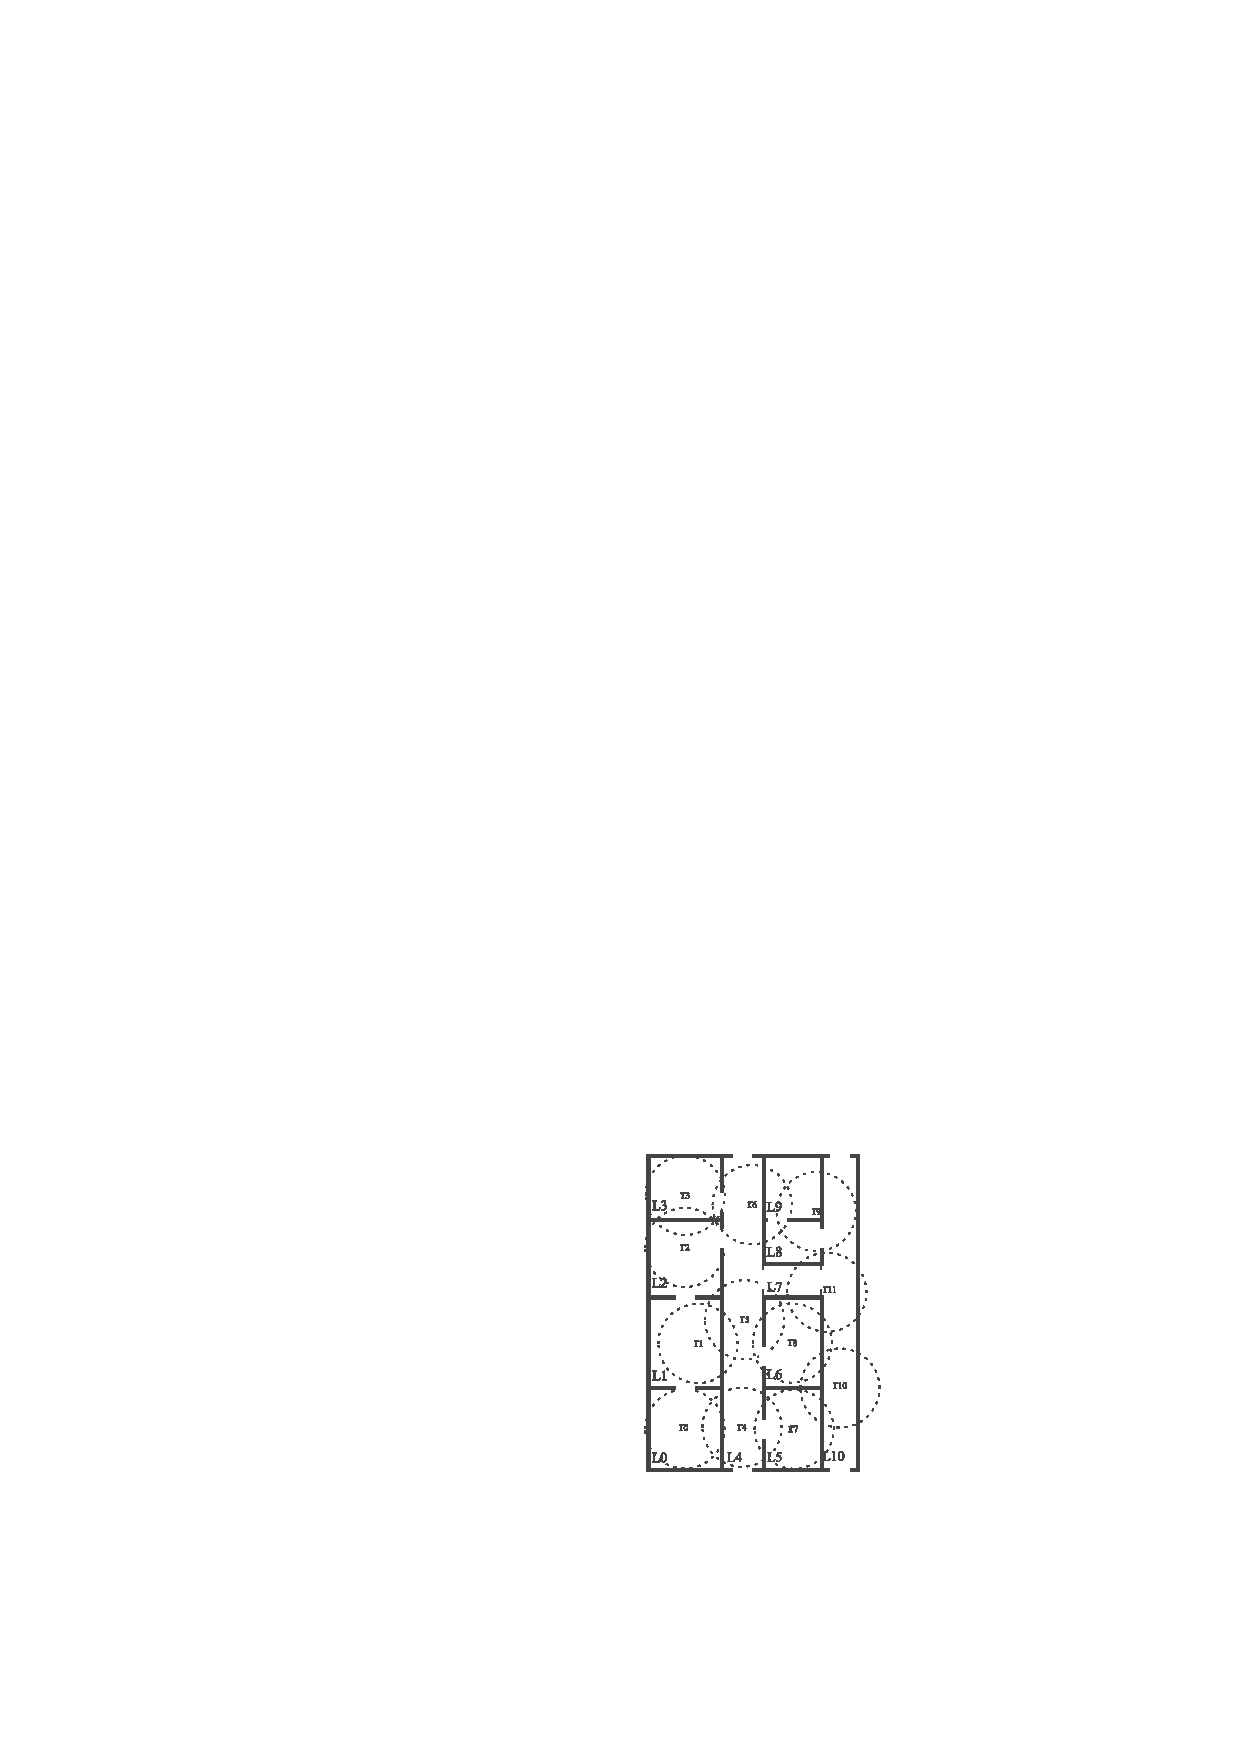
\includegraphics[width=\columnwidth]{figures/3-4/3-4-1.pdf}
  \end{figure}

  \column{0.6\textwidth}
  \begin{example}
    \fsize{
    an object $o$ was detected at some instant by both reader $r_1$ and $r_5$, two locations are possible, $L_1$ and $L_4$. Analogously, if $o$ was detected by $r_3$ only, we cannot conclude that it was surely in $L_3$, as it could be the case that $r_2$ failed to detect it despite it was close enough to its antenna.
    }
  \end{example}

  % \ssize{\textrm{\\this suggests that the association readers/locations can be naturally modeled in probabilistic terms. For instance by a probability distribution $p^a(l|R)$ defined for each location $l$ and set $R$ of readers.}}
  % $p^a(L_1|\{r_1, r_5\}) = p^a(L_4|\{r_1, r_5\}) = 0.5$
  % $p^a(L_0|\{r_0\}) = 1$

\end{columns}

\end{frame}

%------------------------------------------------

\begin{frame}
\frametitle{Ambiguity of RFID Data}

\begin{columns}

  \column{0.4\textwidth}
  \begin{figure}[tb]
    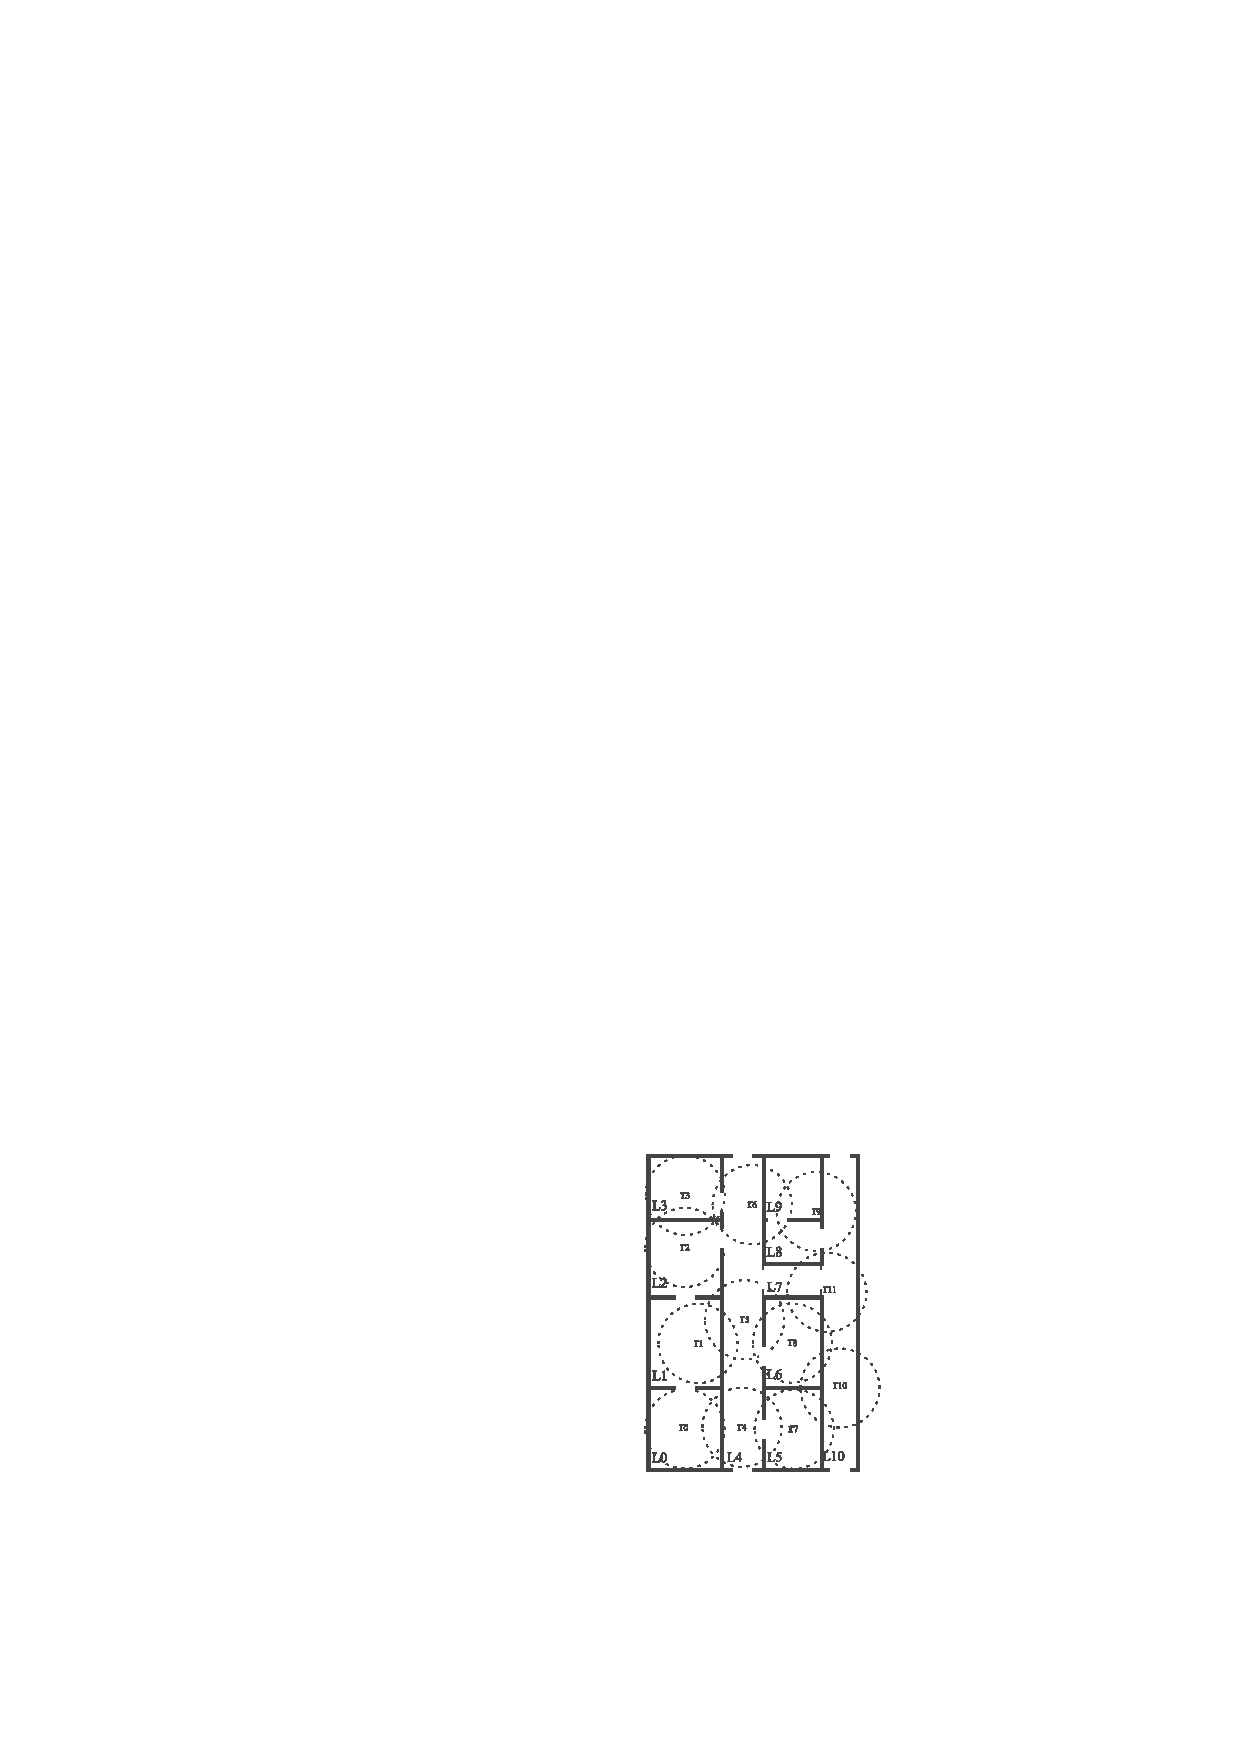
\includegraphics[width=\columnwidth]{figures/3-4/3-4-1.pdf}
  \end{figure}

  \column{0.6\textwidth}
  \begin{figure}[tb]
    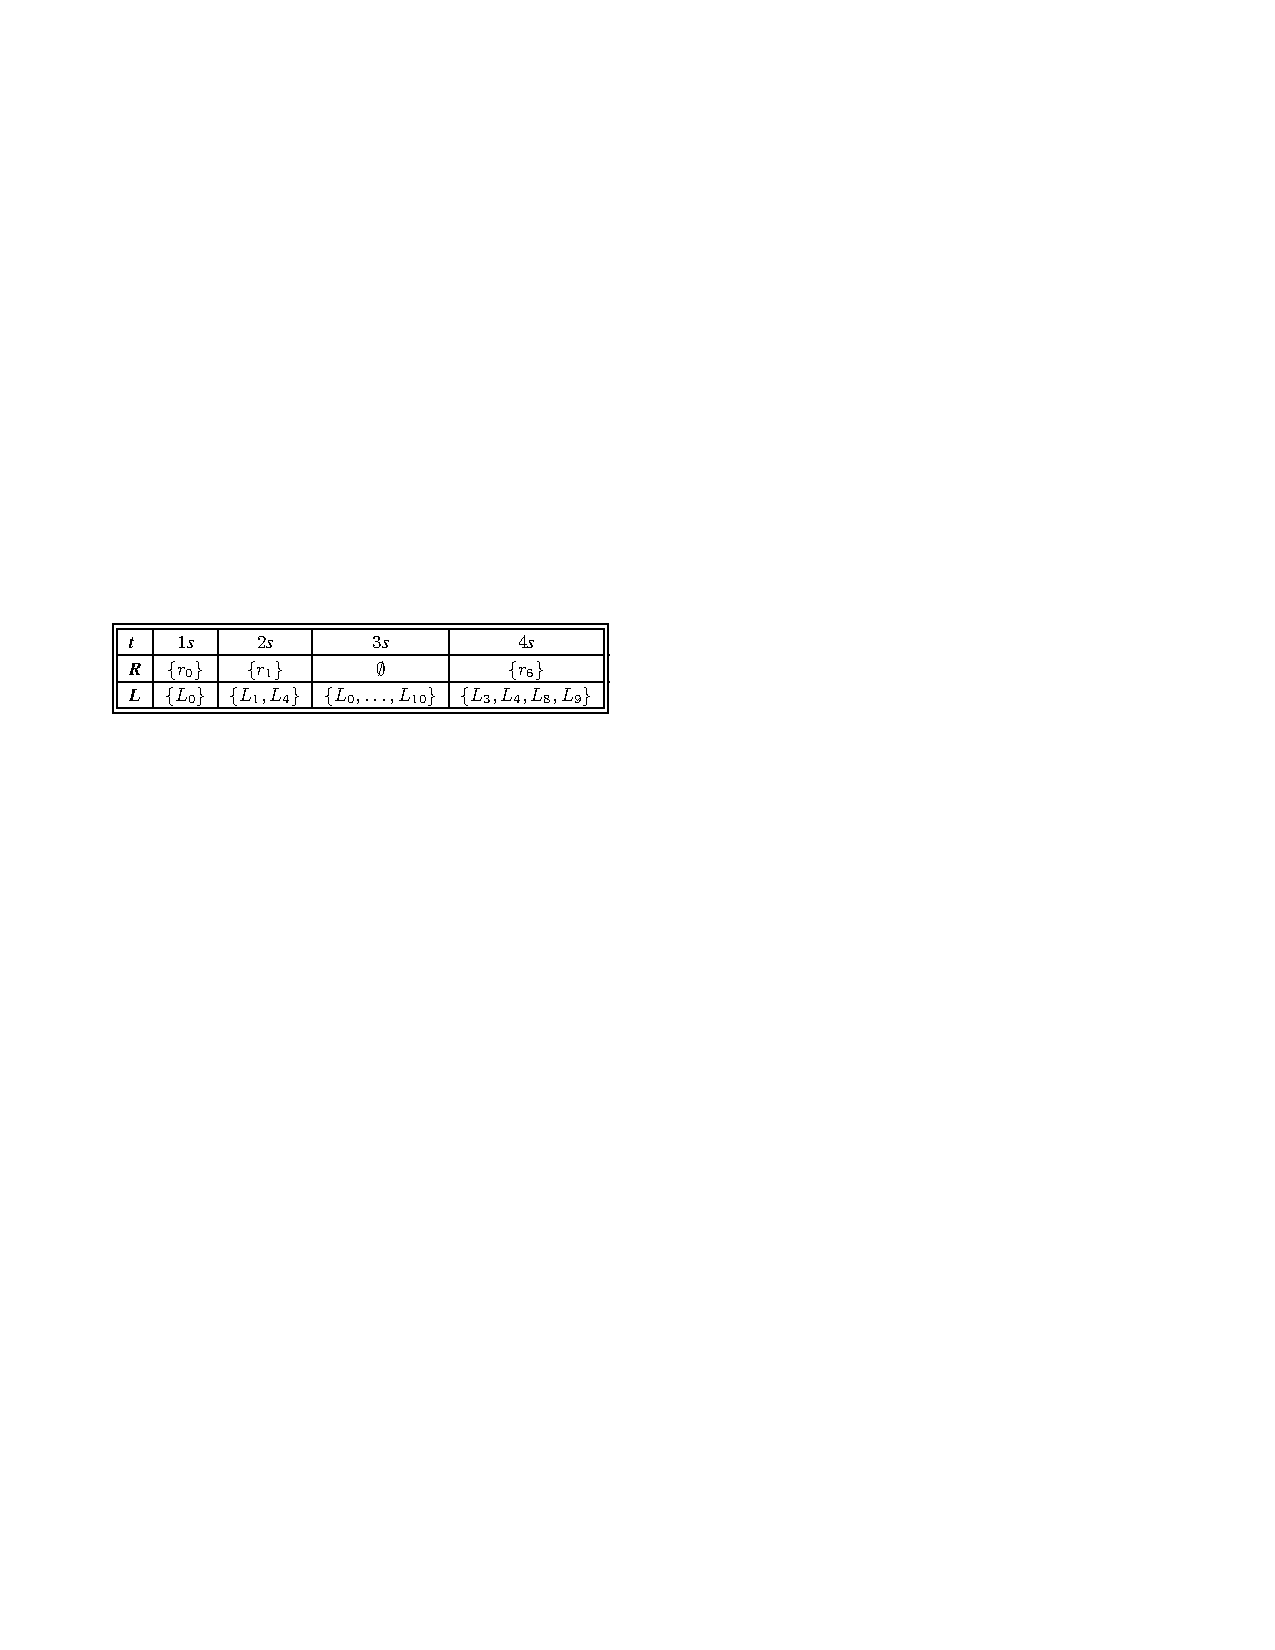
\includegraphics[width=\columnwidth]{figures/3-4/3-4-13.pdf}
  \end{figure}

  \vspace{-10pt}

  \begin{example}
    \ssize{
    $t = 1$: an object detected by $r_0$ is surely at $L_0$ (since the area covered by $r_0$ is totally inside $L_0$)\\
    $t = 2$: an object detected by $r_1$ can be either at $L_1$ or $L_4$ (if object only detected by $r_1$ could also be laid in the area covered by $r_1$ and $r_5$, as $r_5$ may fail to detect the object, the false negative)\\
    $t = 3$: an object detected by no reader can be almost anywhere\\
    $t = 4$: reader $r_6$ covers portions of $L_3, L_4, L_8, L_9$ only.
    }
  \end{example}


\end{columns}

\end{frame}

%------------------------------------------------

\begin{frame}
\frametitle{Ambiguity of RFID Data}

\ssize{\textrm{assume that $o$ is a person, his maximum speed is $v_{max} = 2m/s$. Consider the size of the floor is $15m \times 11m$, re-examine the possible location as follow:}}

\vspace{10pt}

\begin{columns}

  \column{0.3\textwidth}
  \begin{figure}[tb]
    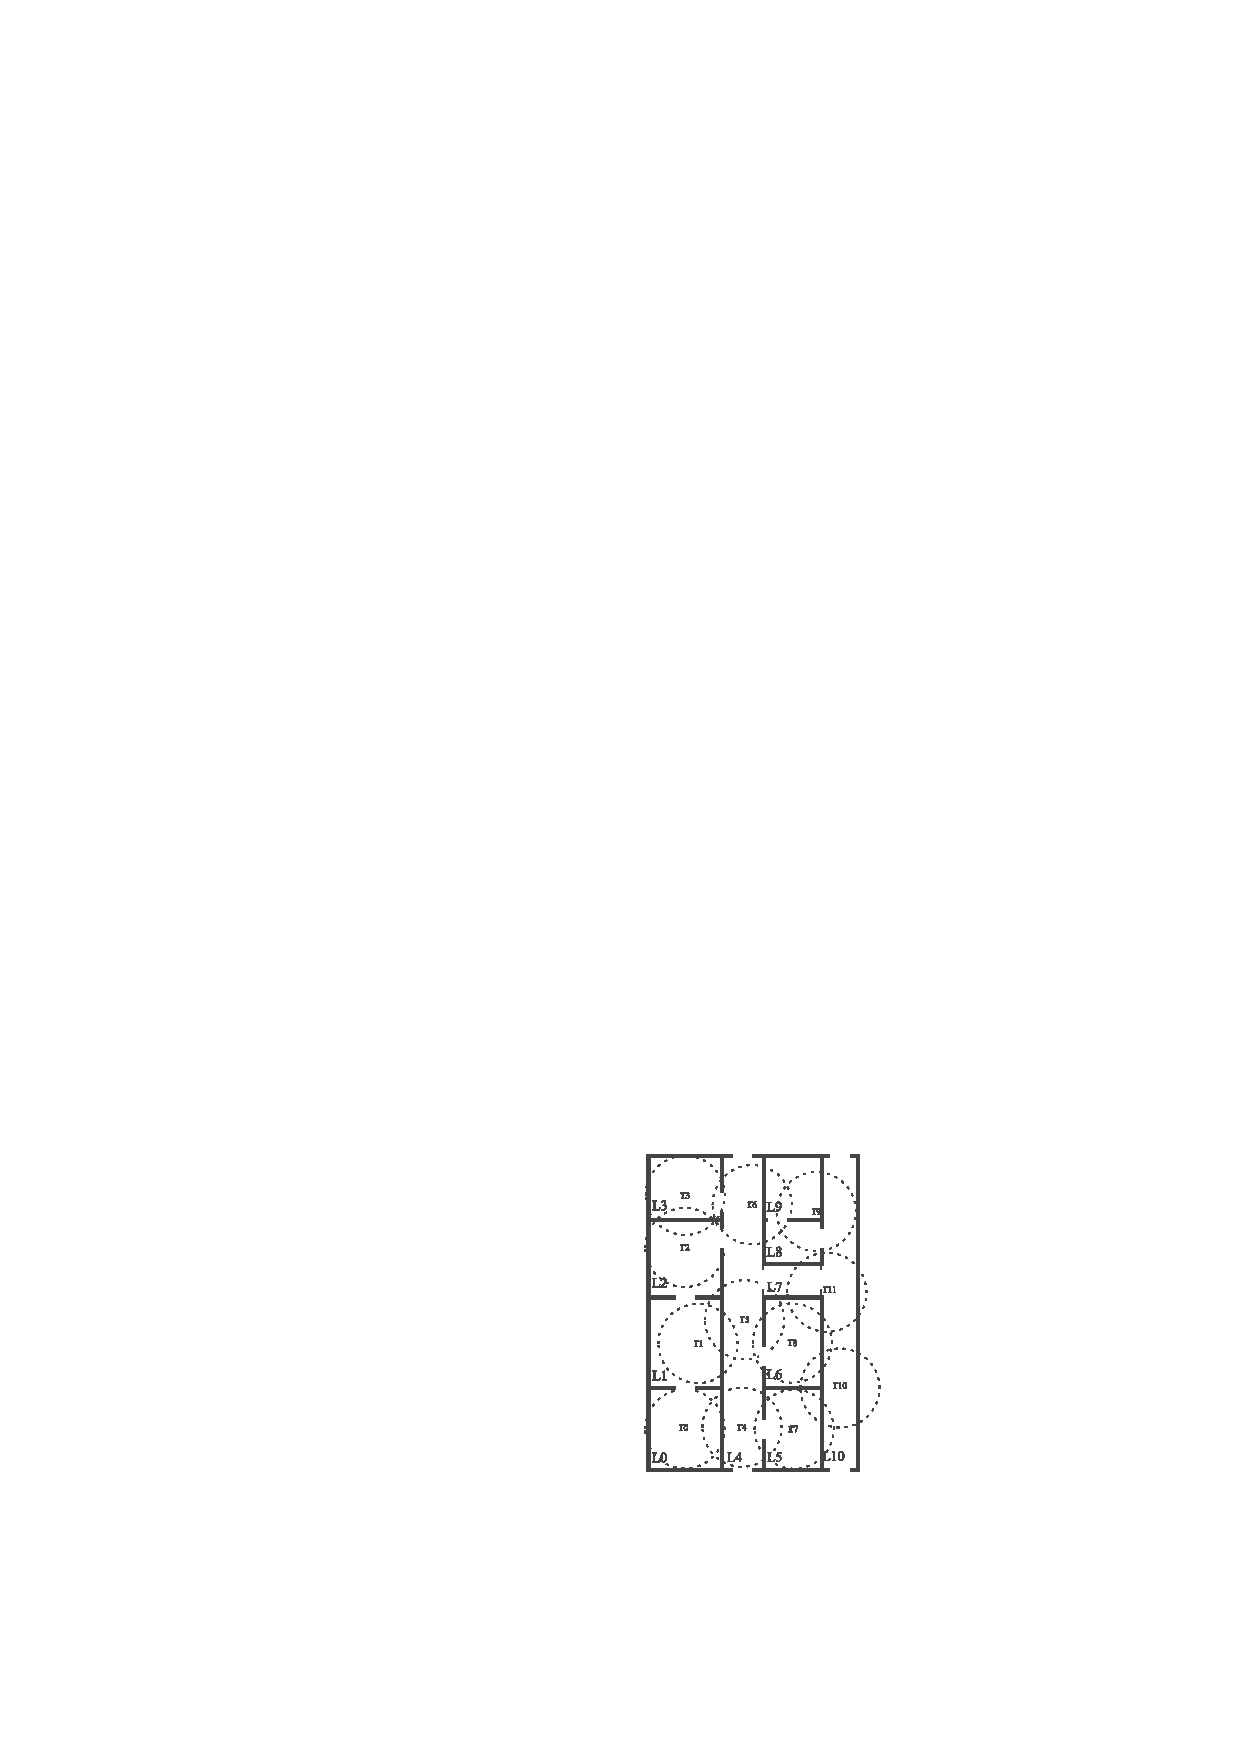
\includegraphics[width=\columnwidth]{figures/3-4/3-4-1.pdf}
  \end{figure}


  \column{0.7\textwidth}
  \ssize{
  A.  As regards $t = 2s$, $o$ must be at $L_1$, as it cannot be at $L_4$. In fact, $o$ was at $L_0$ at $t = 1s$, and the minimum (indoor) distance between $L_0$ and $L_4$ (about 7m) cannot be covered in $1sec$ without exceeding $v_{max}$. \\~\\
  B.  As regards $t = 3s$, now that it has been established that $o$ was at $L_1$ at $t = 2s$, we can restrict the set of possbile locations from $\{ L_1,...,L_{10} \}$ to $\{ L_0, L_1, L_2 \}$ (due to the size of the floor, reaching a room not in this set from any position inside $L_1$ in one second would require a speed greater than $v_{max}$). \\~\\
  C.  As regards $t = 4s$, the only location in $\{ L_3, L_4, L_8, L_9 \}$ (the set of location covered by $r_6$) that can be reached from at least one location in $\{ L_0, L_1, L_2 \}$ (the possible locations at time $t = 3s$, as established at point B) is $L_4$.
  }


\end{columns}

\end{frame}

%------------------------------------------------

\begin{frame}
\frametitle{Ambiguity of RFID Data}

\ssize{\textrm{all the arguments used in Point A,B,C show that the exploiting the correlation with the past positions can reduce (or even eliminate) the uncertainty in determining the position at any time point. Trying to further reduce the uncertainty by exploiting the correlation:}}

\vspace{10pt}

\begin{columns}

  \column{0.3\textwidth}
  \begin{figure}[tb]
    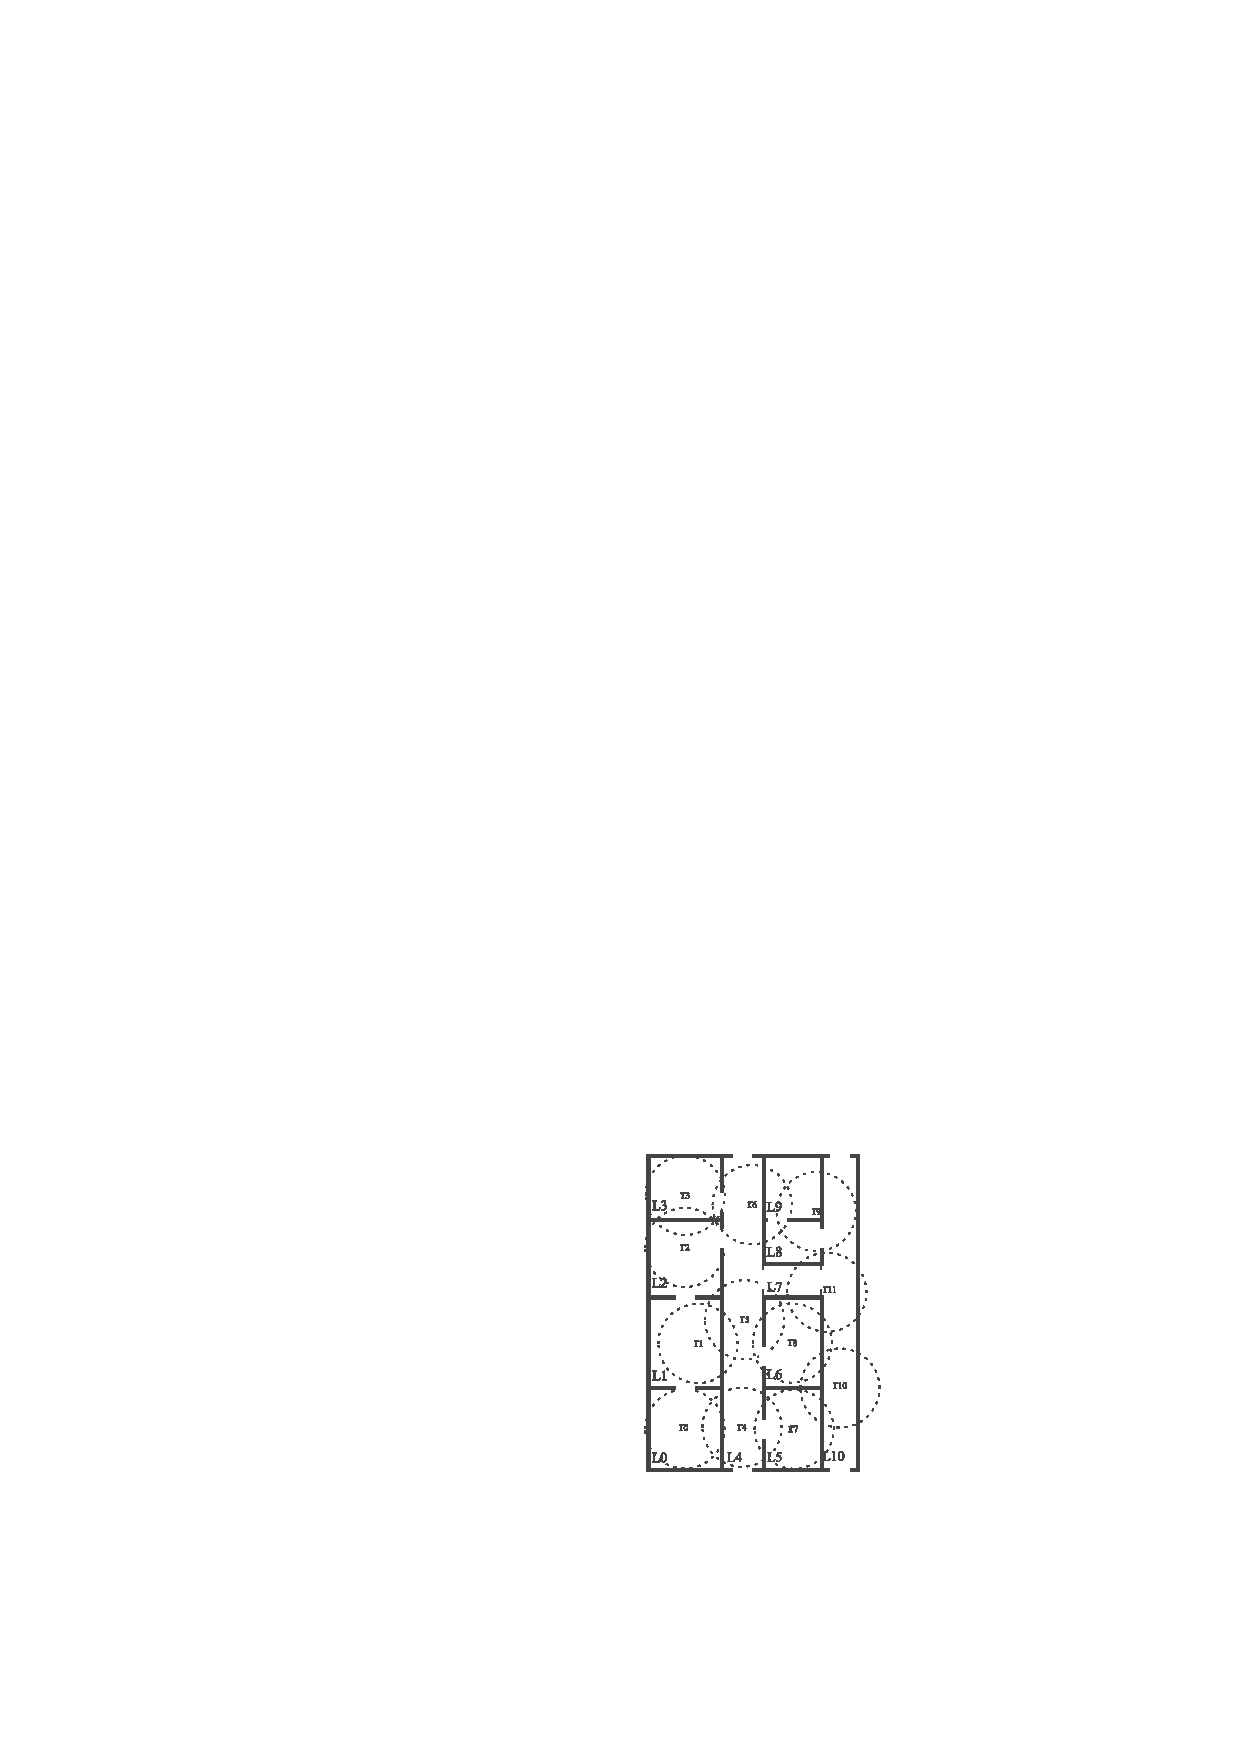
\includegraphics[width=\columnwidth]{figures/3-4/3-4-1.pdf}
  \end{figure}


  \column{0.7\textwidth}
  \ssize{
  D.  Consider $t = 3s$, we have already established that the position of $o$ at the subsequent time point is $L_4$, and that the possible locations for this time point are $L_0, L_1, L_2$. Hence, at $t = 3s$, $o$ must have been at $L_2$, as this is the only among the possible locations for this time point from which $L_4$ can be reached in one second without exceeding $v_{max}$.
  }

  \begin{figure}[tb]
    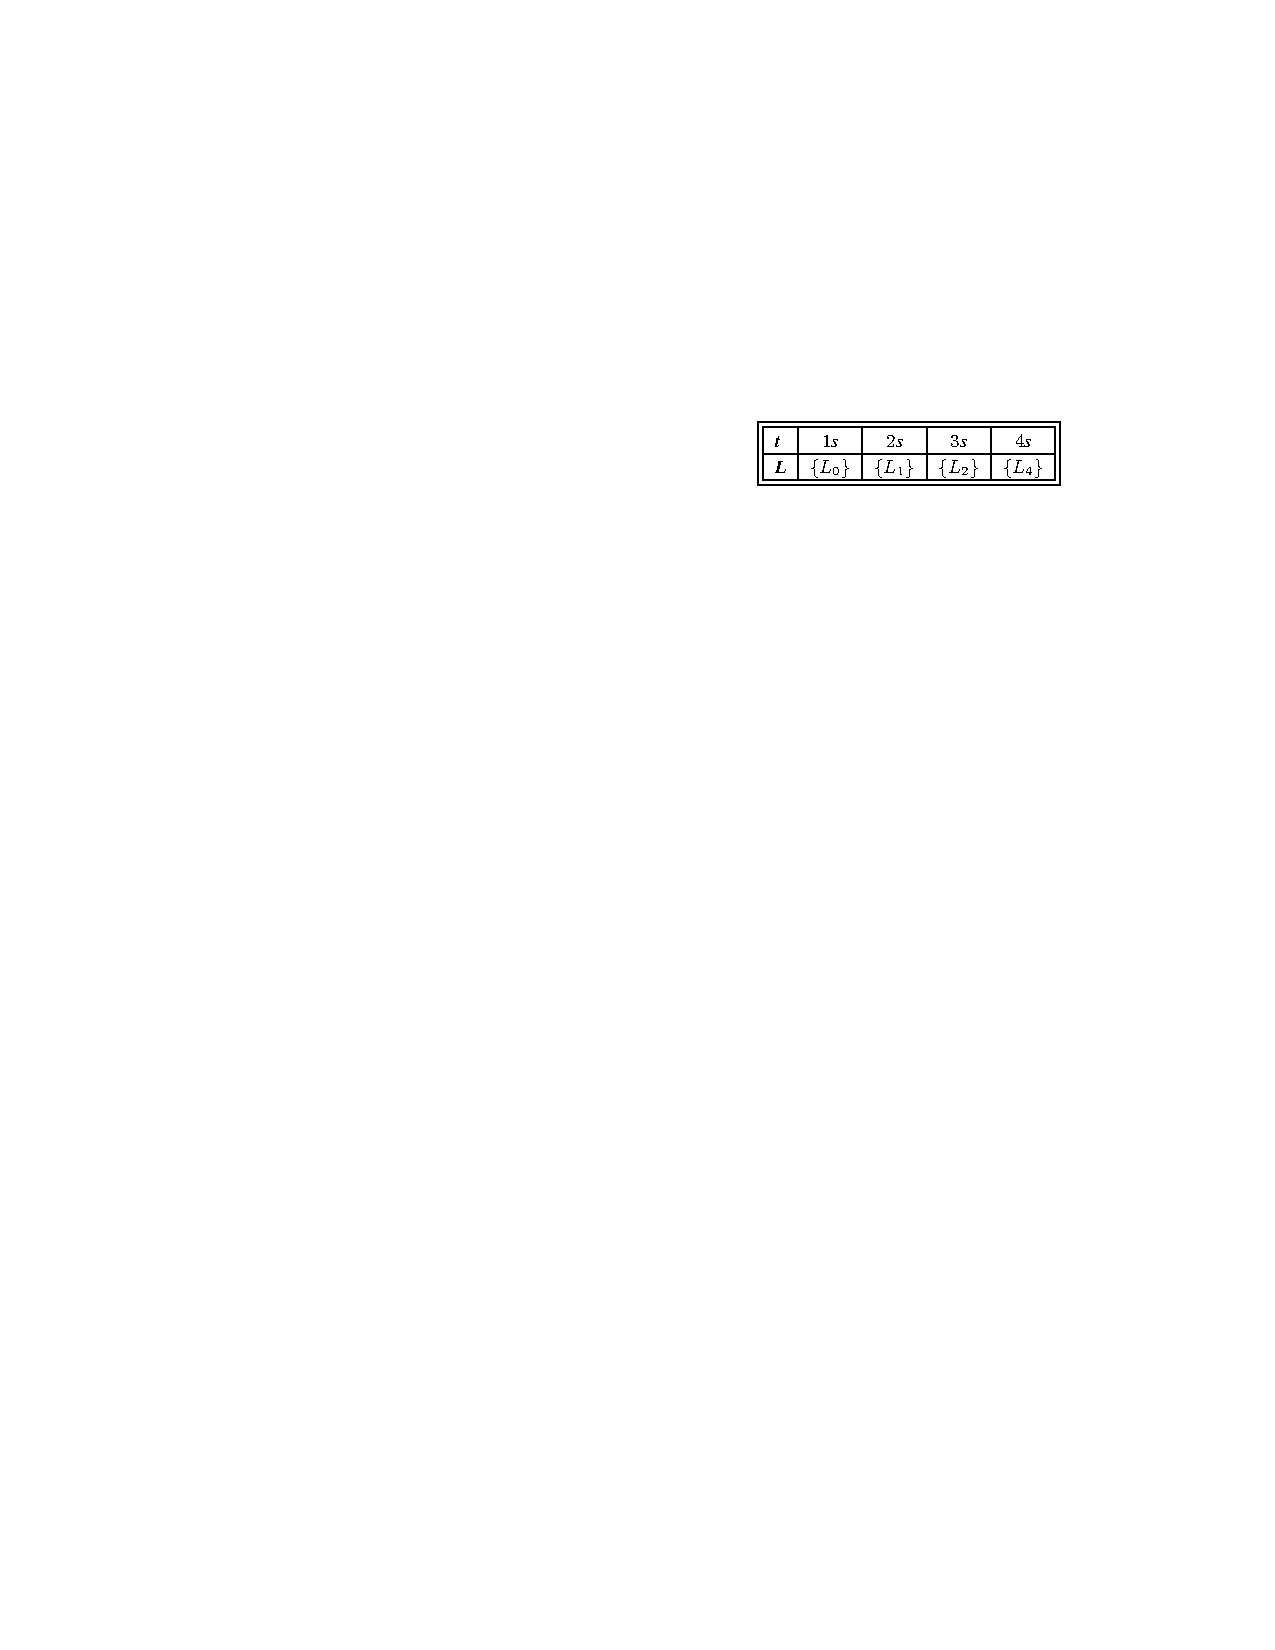
\includegraphics[width=\columnwidth]{figures/3-4/3-4-14.pdf}
  \end{figure}


\end{columns}

\end{frame}

%------------------------------------------------

\begin{frame}
\frametitle{The Problem Setting for This Work}

\fsize{

An instance of \conceptbf{smoothing problem}~\cite{smith2013sequential}: estimating the state of an observed entity at a time point $t \in [1...T]$ on the basis of all the observations over $[1...T]$ in terms of a posterior probability distribution over the possible states.\\~\\

This work proposes a smoothing technique following a two-way-filtering scheme that embeds a sampling strategy for efficiently dealing with missing detections.\\~\\

In the first \emph{forward} phase, time points are processed from the first to the last, and the possible positions at each time point are filtered by taking into account the results of the previous steps.\\~\\

In the \emph{backward} phase, it proceeds from the last to the first time point: for each time point, filter the positions detected as admissible in the forward phase and revise their weights, by checking whether they are a valid position when looking at the results obtained for the future time point.

}

\end{frame}

%------------------------------------------------

\begin{frame}
\frametitle{The Problem Setting for This Work}

\fsize{

The map of the locations is assumed to be partitioned according to a grid, thus the positions to be filtered and weighted at each step of the forward phase are the grid cells compatible with the readers that performed the detection.\\~\\

Thus, the grid cells may result in too many candidate positions, a variant of the cleaning algorithm where missing detections are treated by integrating the grid-based approach with sampling strategy is proposed.\\~\\

At the end of each forward step involving a missing detection, the cells that survived the filtering are further filtered according to a sampling technique, where the probability of a cell to be sampled is an estimate of the probability it would have been assigned if it was considered also in the following phases.

}

\end{frame}
